\documentclass{article}
\usepackage[utf8]{inputenc}
\usepackage{geometry}
 \geometry{
 a4paper,
 total={170mm,257mm},
 left=20mm,
 top=20mm,
 }
 \usepackage{graphicx}
 \usepackage{subcaption}
 \usepackage{titling}
 \usepackage{float}

 \title{ASSIGNMENT 2: Computer Vision 792}
\author{Madhia Shabih}
\date{August 2024}
 
 \usepackage{fancyhdr}
\fancypagestyle{plain}{%  the preset of fancyhdr 
    \fancyhf{} % clear all header and footer fields
    \fancyfoot[L]{\thedate}
    \fancyhead[L]{24397644}
    \fancyhead[R]{\theauthor}
}
\makeatletter
\def\@maketitle{%
  \newpage
  \null
  \vskip 1em%
  \begin{center}%
  \let \footnote \thanks
    {\LARGE \@title \par}%
    \vskip 1em%
    %{\large \@date}%
  \end{center}%
  \par
  \vskip 1em}
\makeatother

\usepackage{lipsum}  
\usepackage{cmbright}

\begin{document}
\maketitle
\section{Question 1}
\begin{figure}[H]
    \centering
    \begin{subfigure}{.3\textwidth}
        \centering
        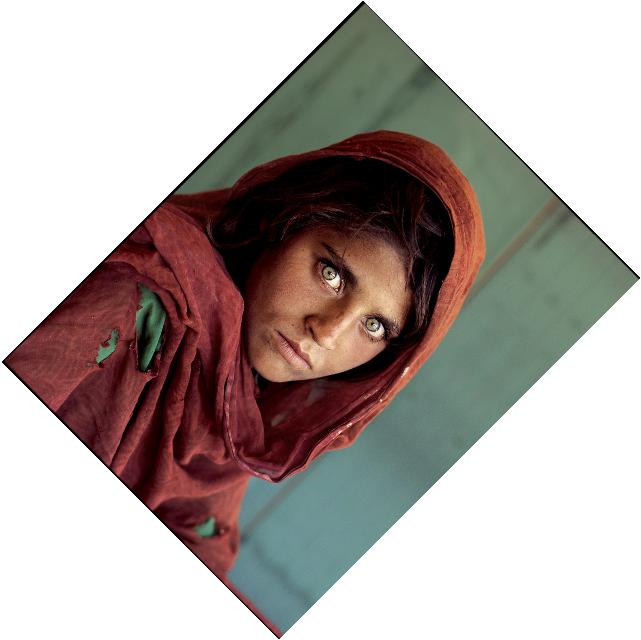
\includegraphics[scale=0.04]{q1/output/similar_0.5_0.5_2.jpg}
        \subcaption{}
    \end{subfigure}
    \begin{subfigure}{.3\textwidth}
        \centering
        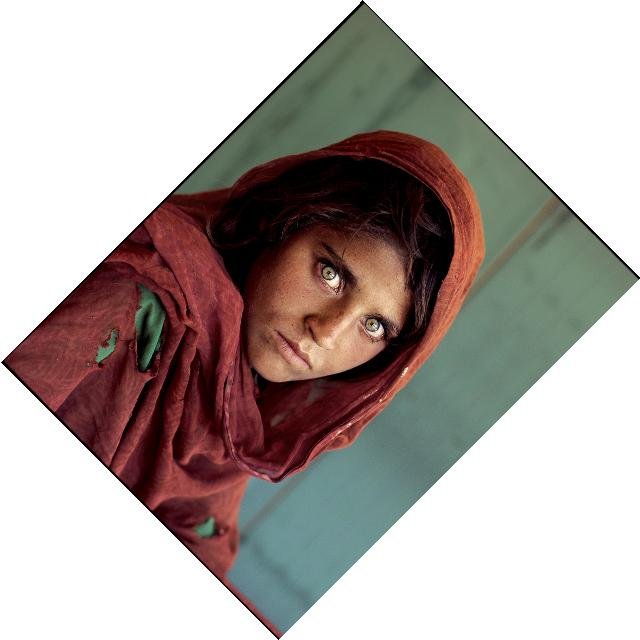
\includegraphics[scale=0.04]{q1/output/similar_0.5_1_2.jpg}
        \subcaption{}
    \end{subfigure}
    \begin{subfigure}{.3\textwidth}
        \centering
        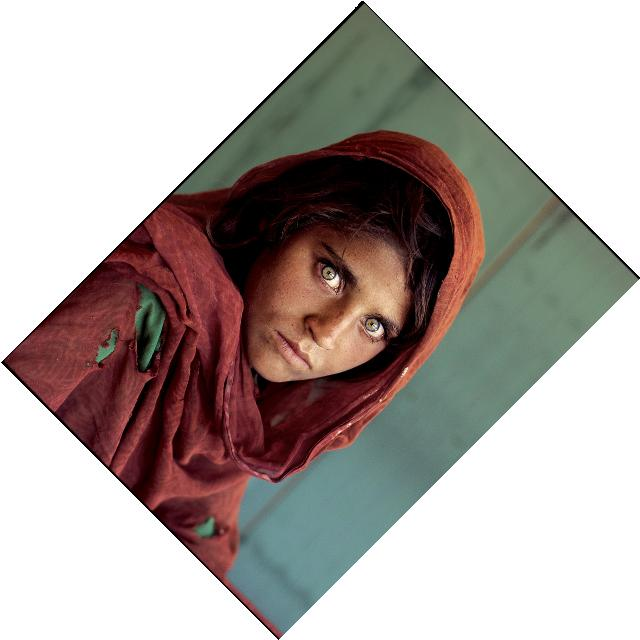
\includegraphics[scale=0.04]{q1/output/similar_0.5_2_2.jpg}
        \subcaption{}
    \end{subfigure}
    \caption{(a) blah (b) blah (c) blah}
\end{figure}

\begin{figure}[H]
    \centering
    \begin{subfigure}{.3\textwidth}
        \centering
        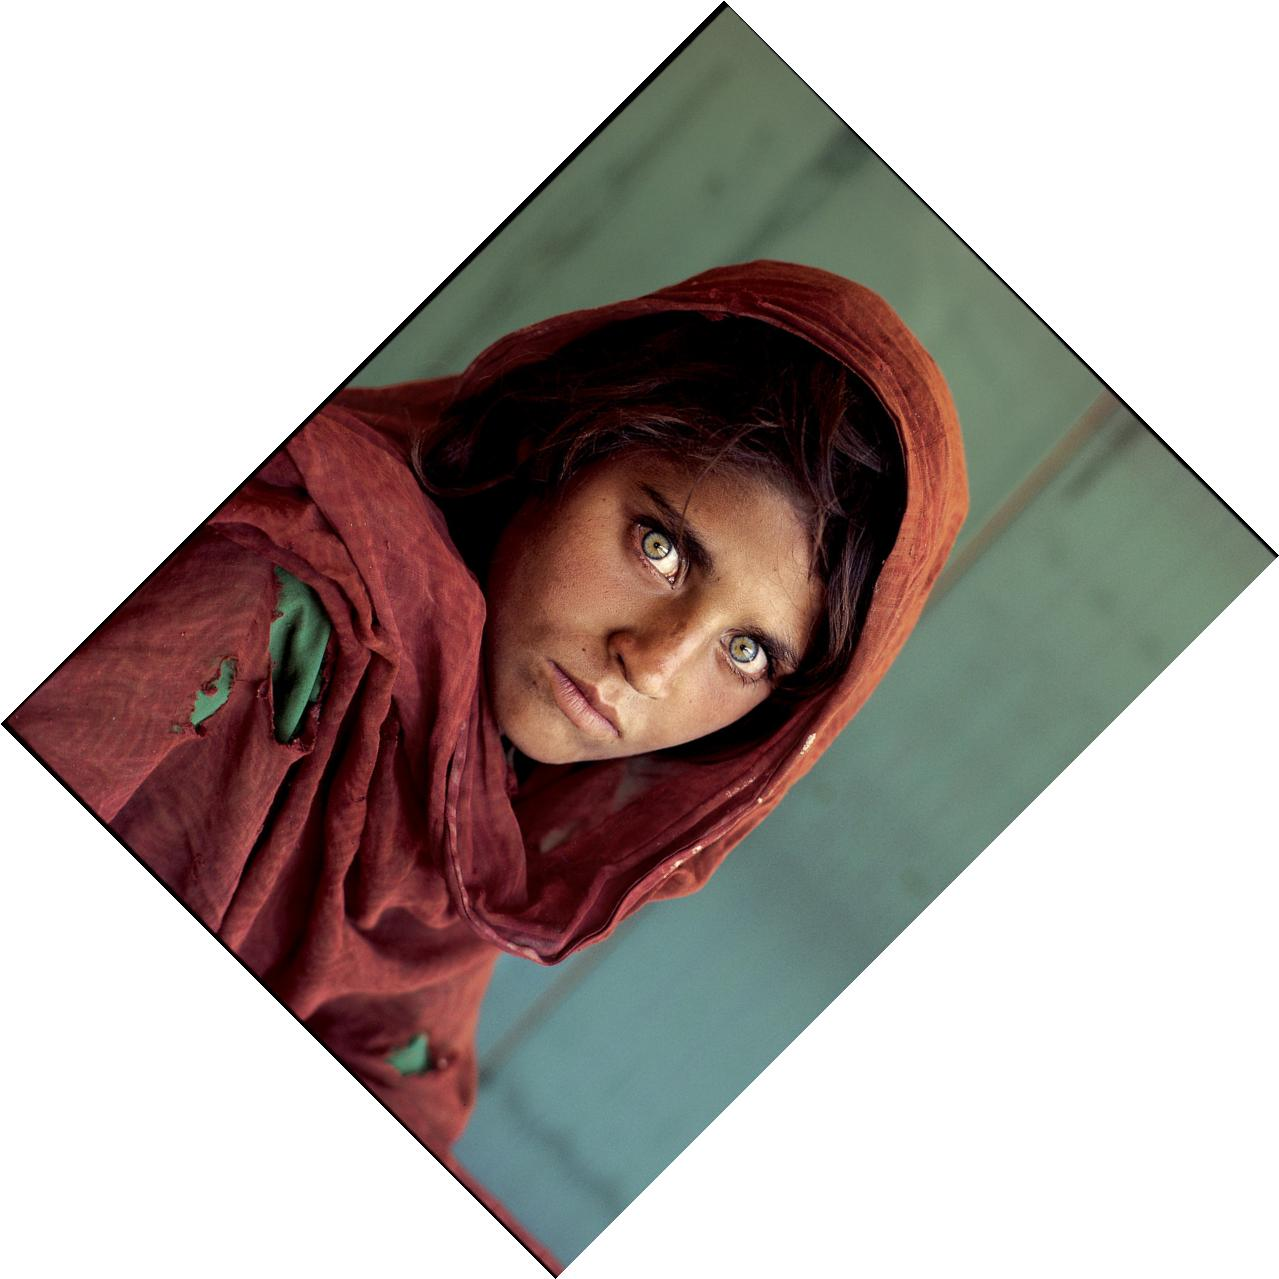
\includegraphics[scale=0.04]{q1/output/similar_1_0.5_2.jpg}
        \subcaption{}
    \end{subfigure}
    \begin{subfigure}{.3\textwidth}
        \centering
        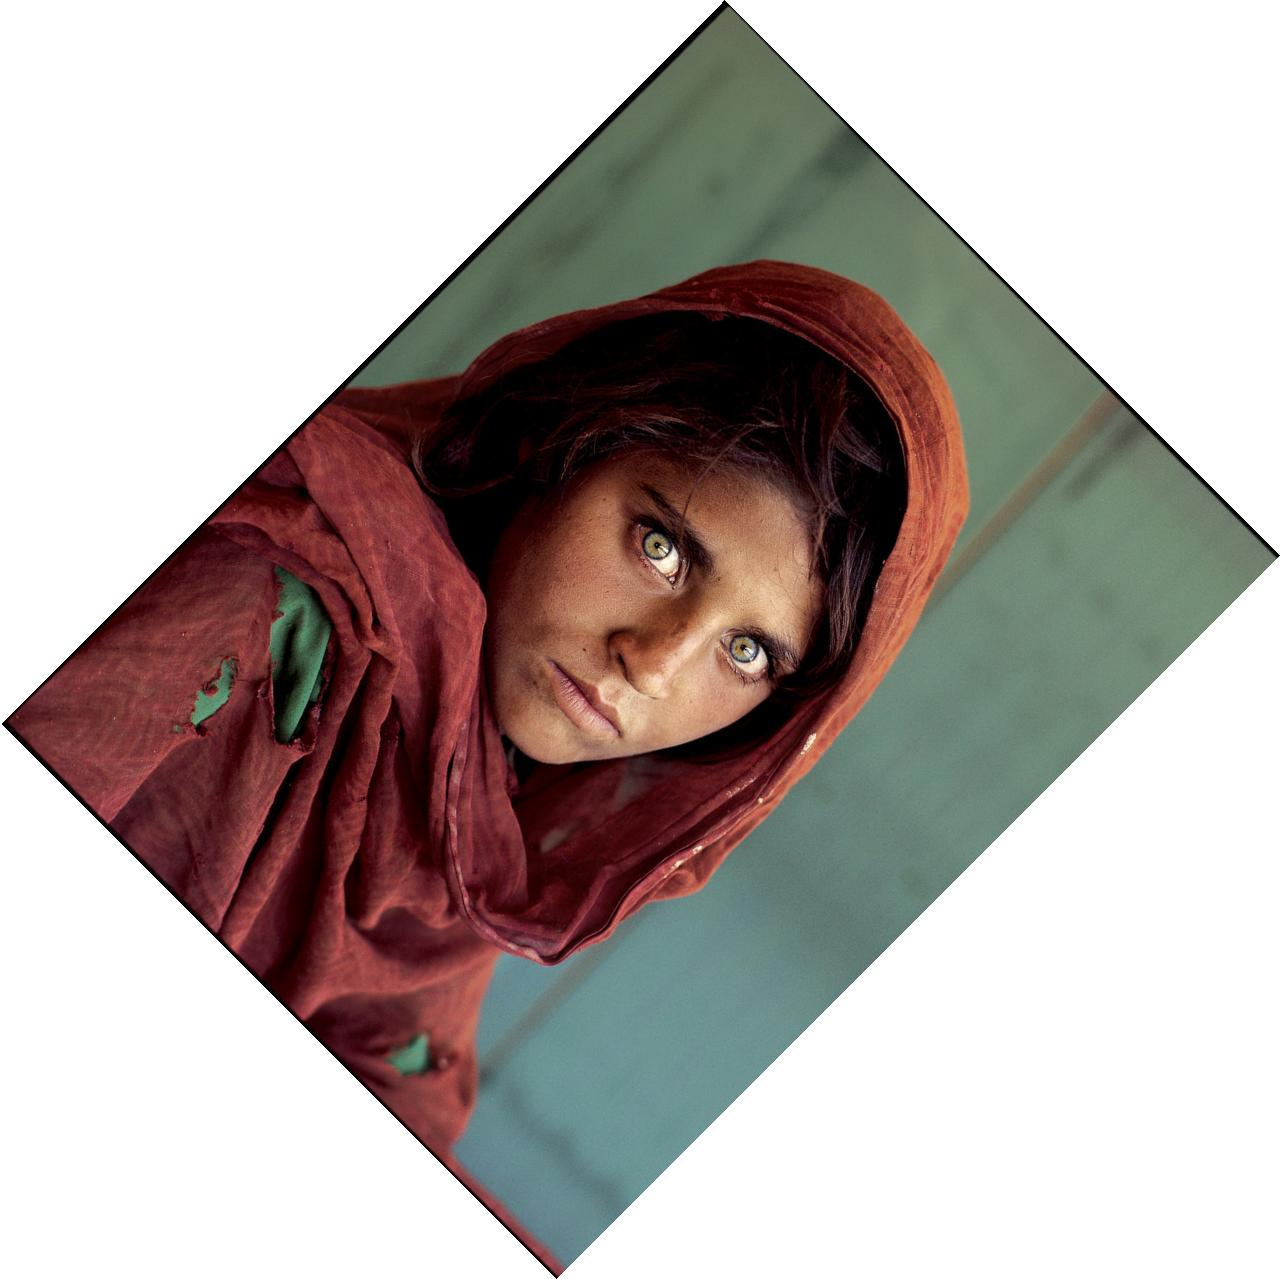
\includegraphics[scale=0.04]{q1/output/similar_1_1_2.jpg}
        \subcaption{}
    \end{subfigure}
    \begin{subfigure}{.3\textwidth}
        \centering
        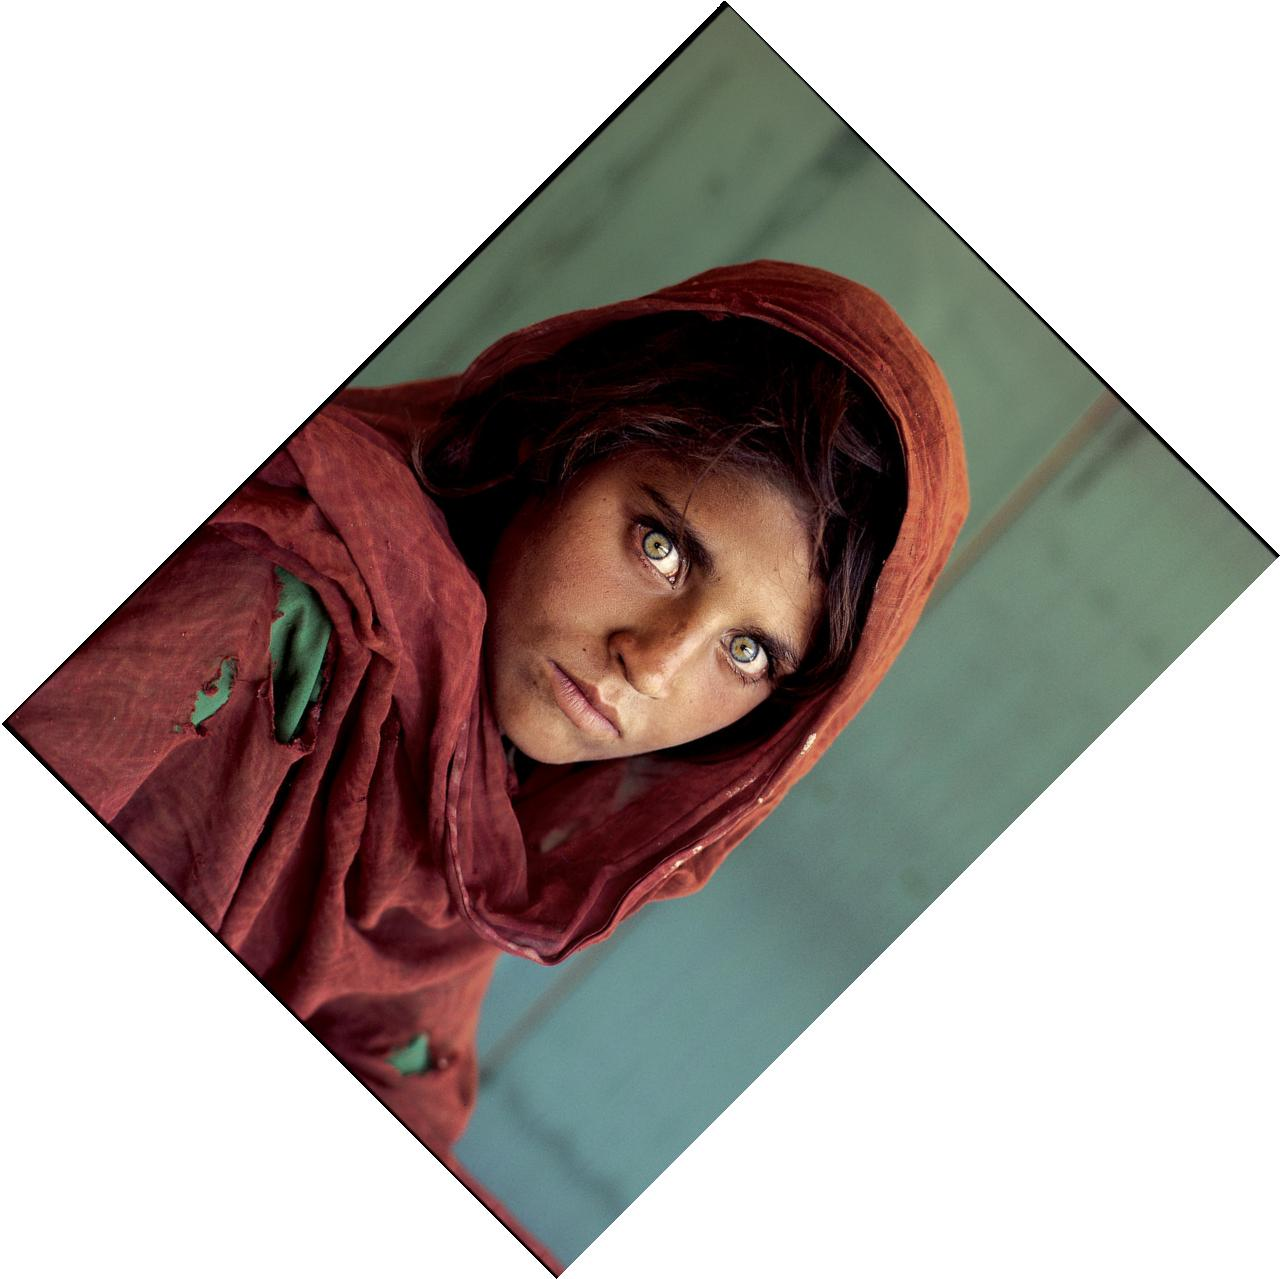
\includegraphics[scale=0.04]{q1/output/similar_1_2_2.jpg}
        \subcaption{}
    \end{subfigure}
    \caption{(a) blah (b) blah (c) blah}
\end{figure}

\begin{figure}[H]
    \centering
    \begin{subfigure}{.3\textwidth}
        \centering
        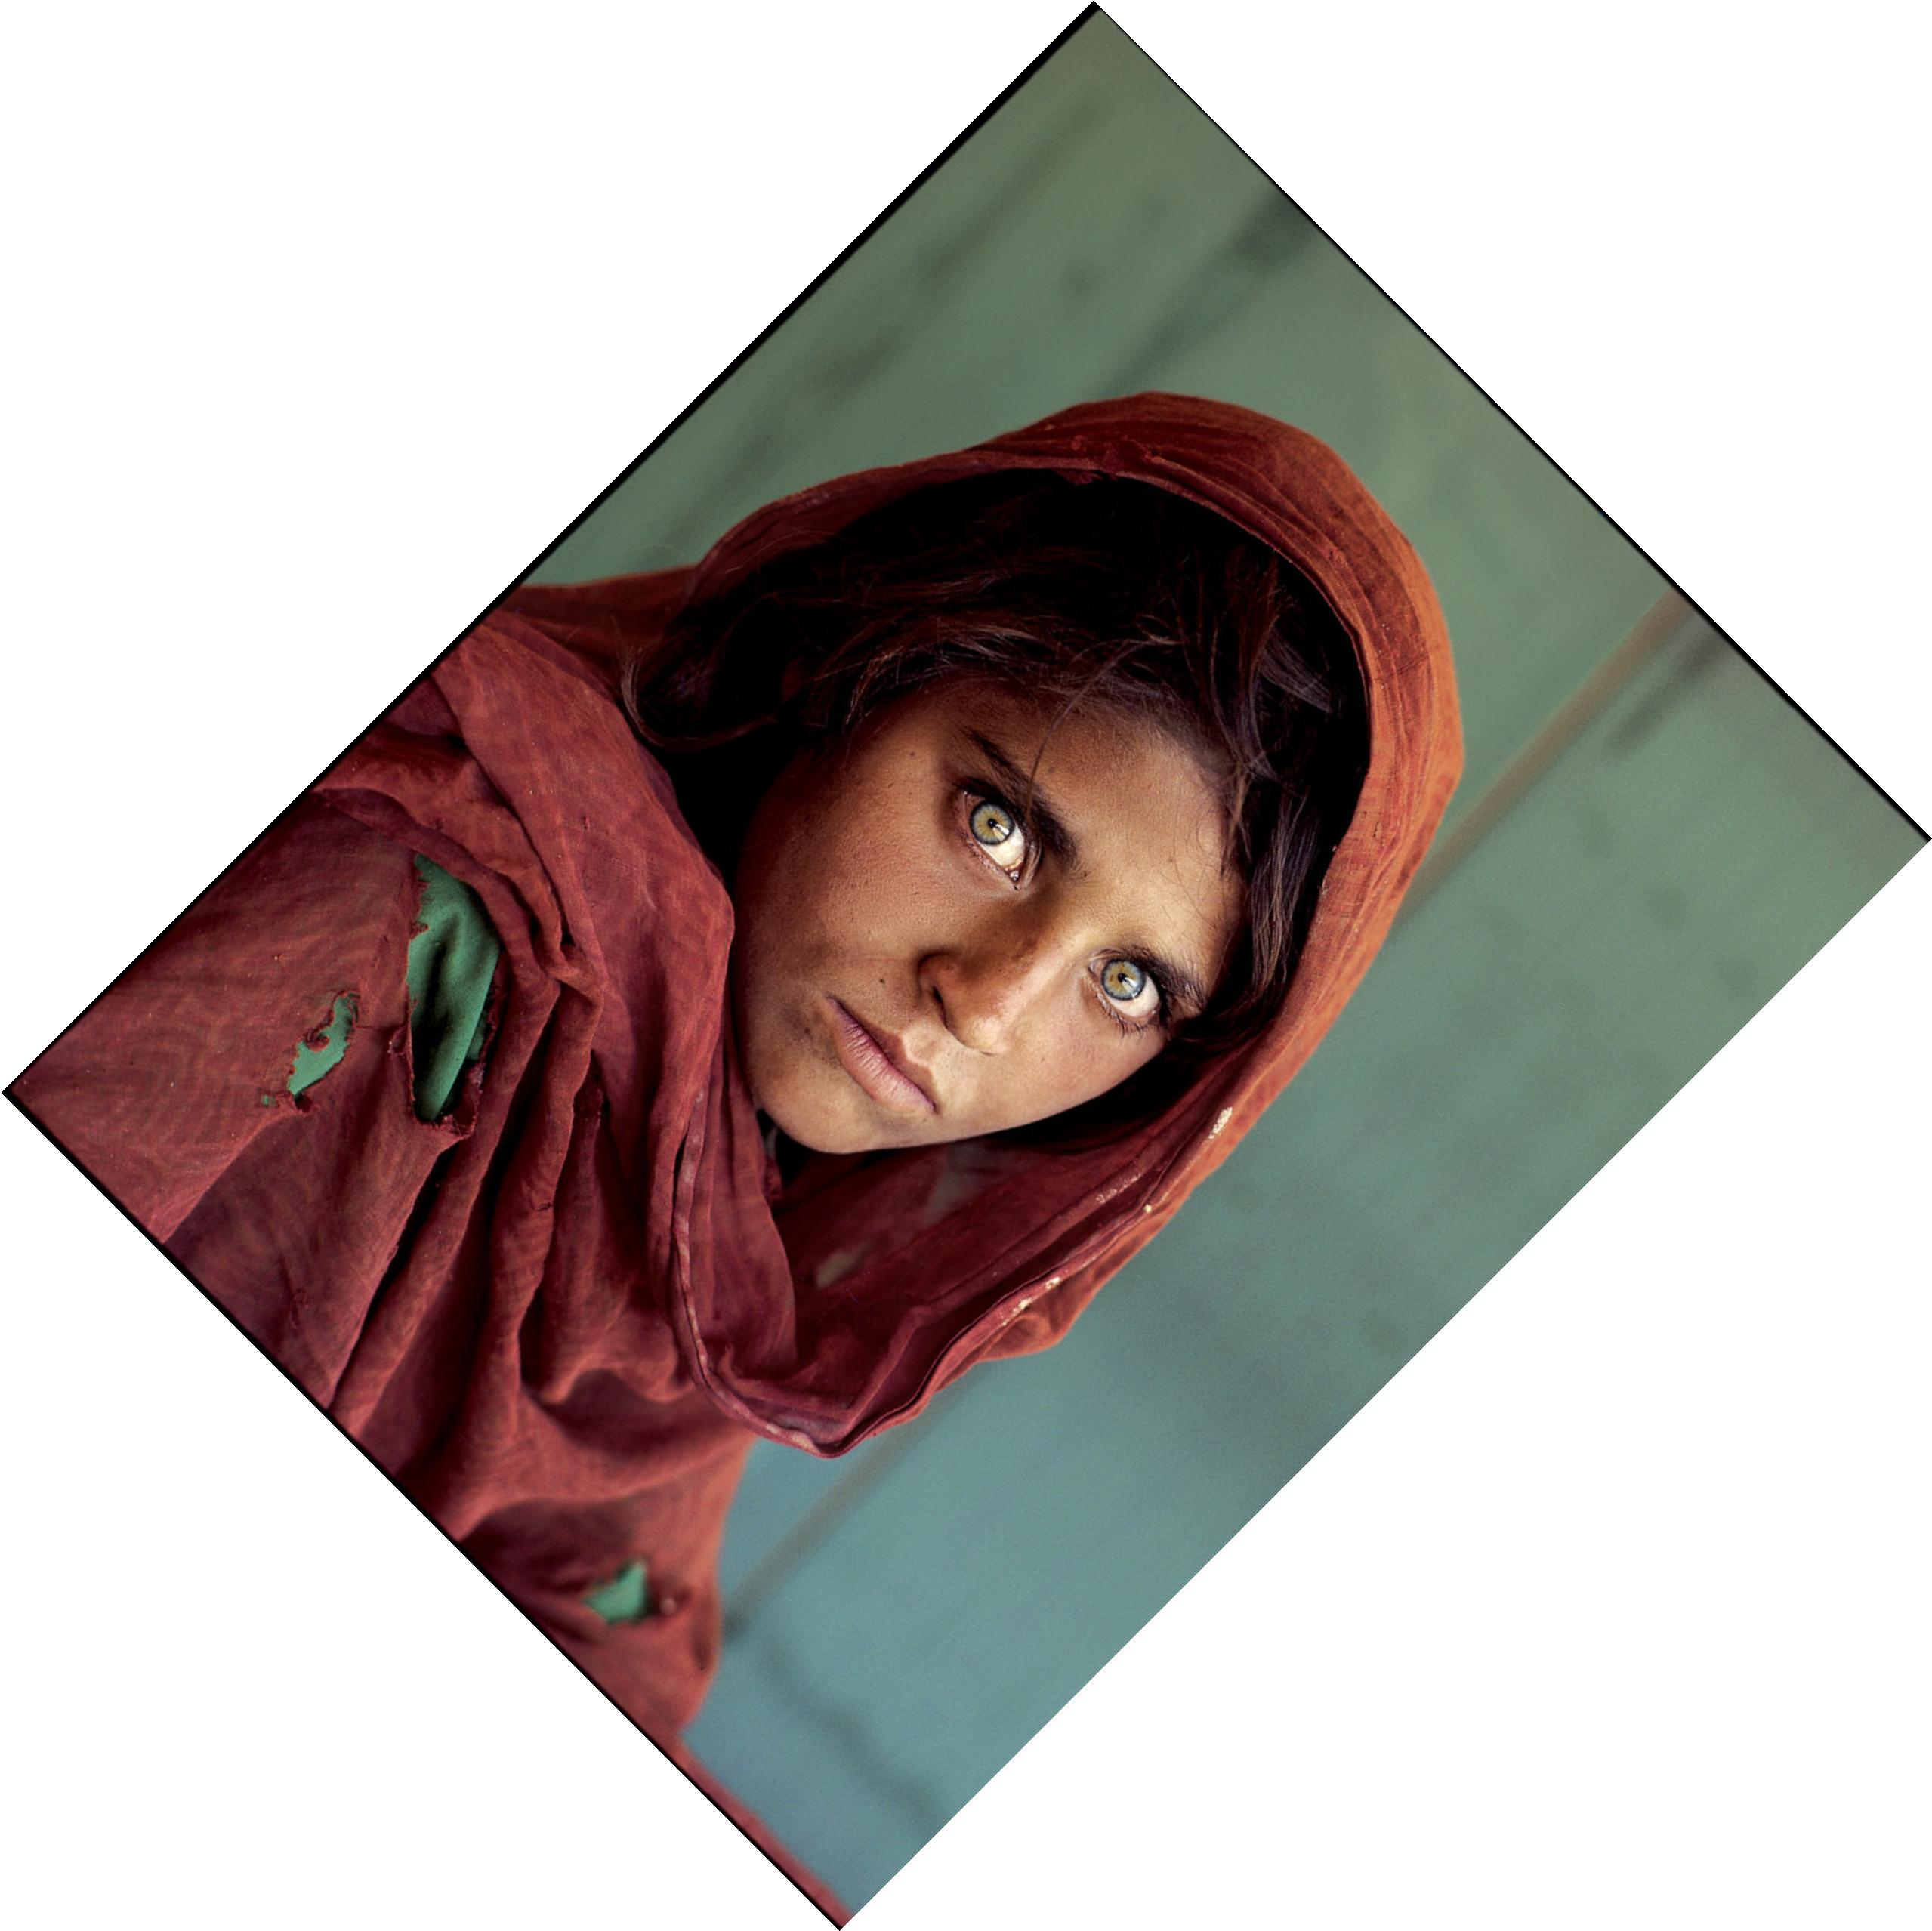
\includegraphics[scale=0.04]{q1/output/similar_2_0.5_2.jpg}
        \subcaption{}
    \end{subfigure}
    \begin{subfigure}{.3\textwidth}
        \centering
        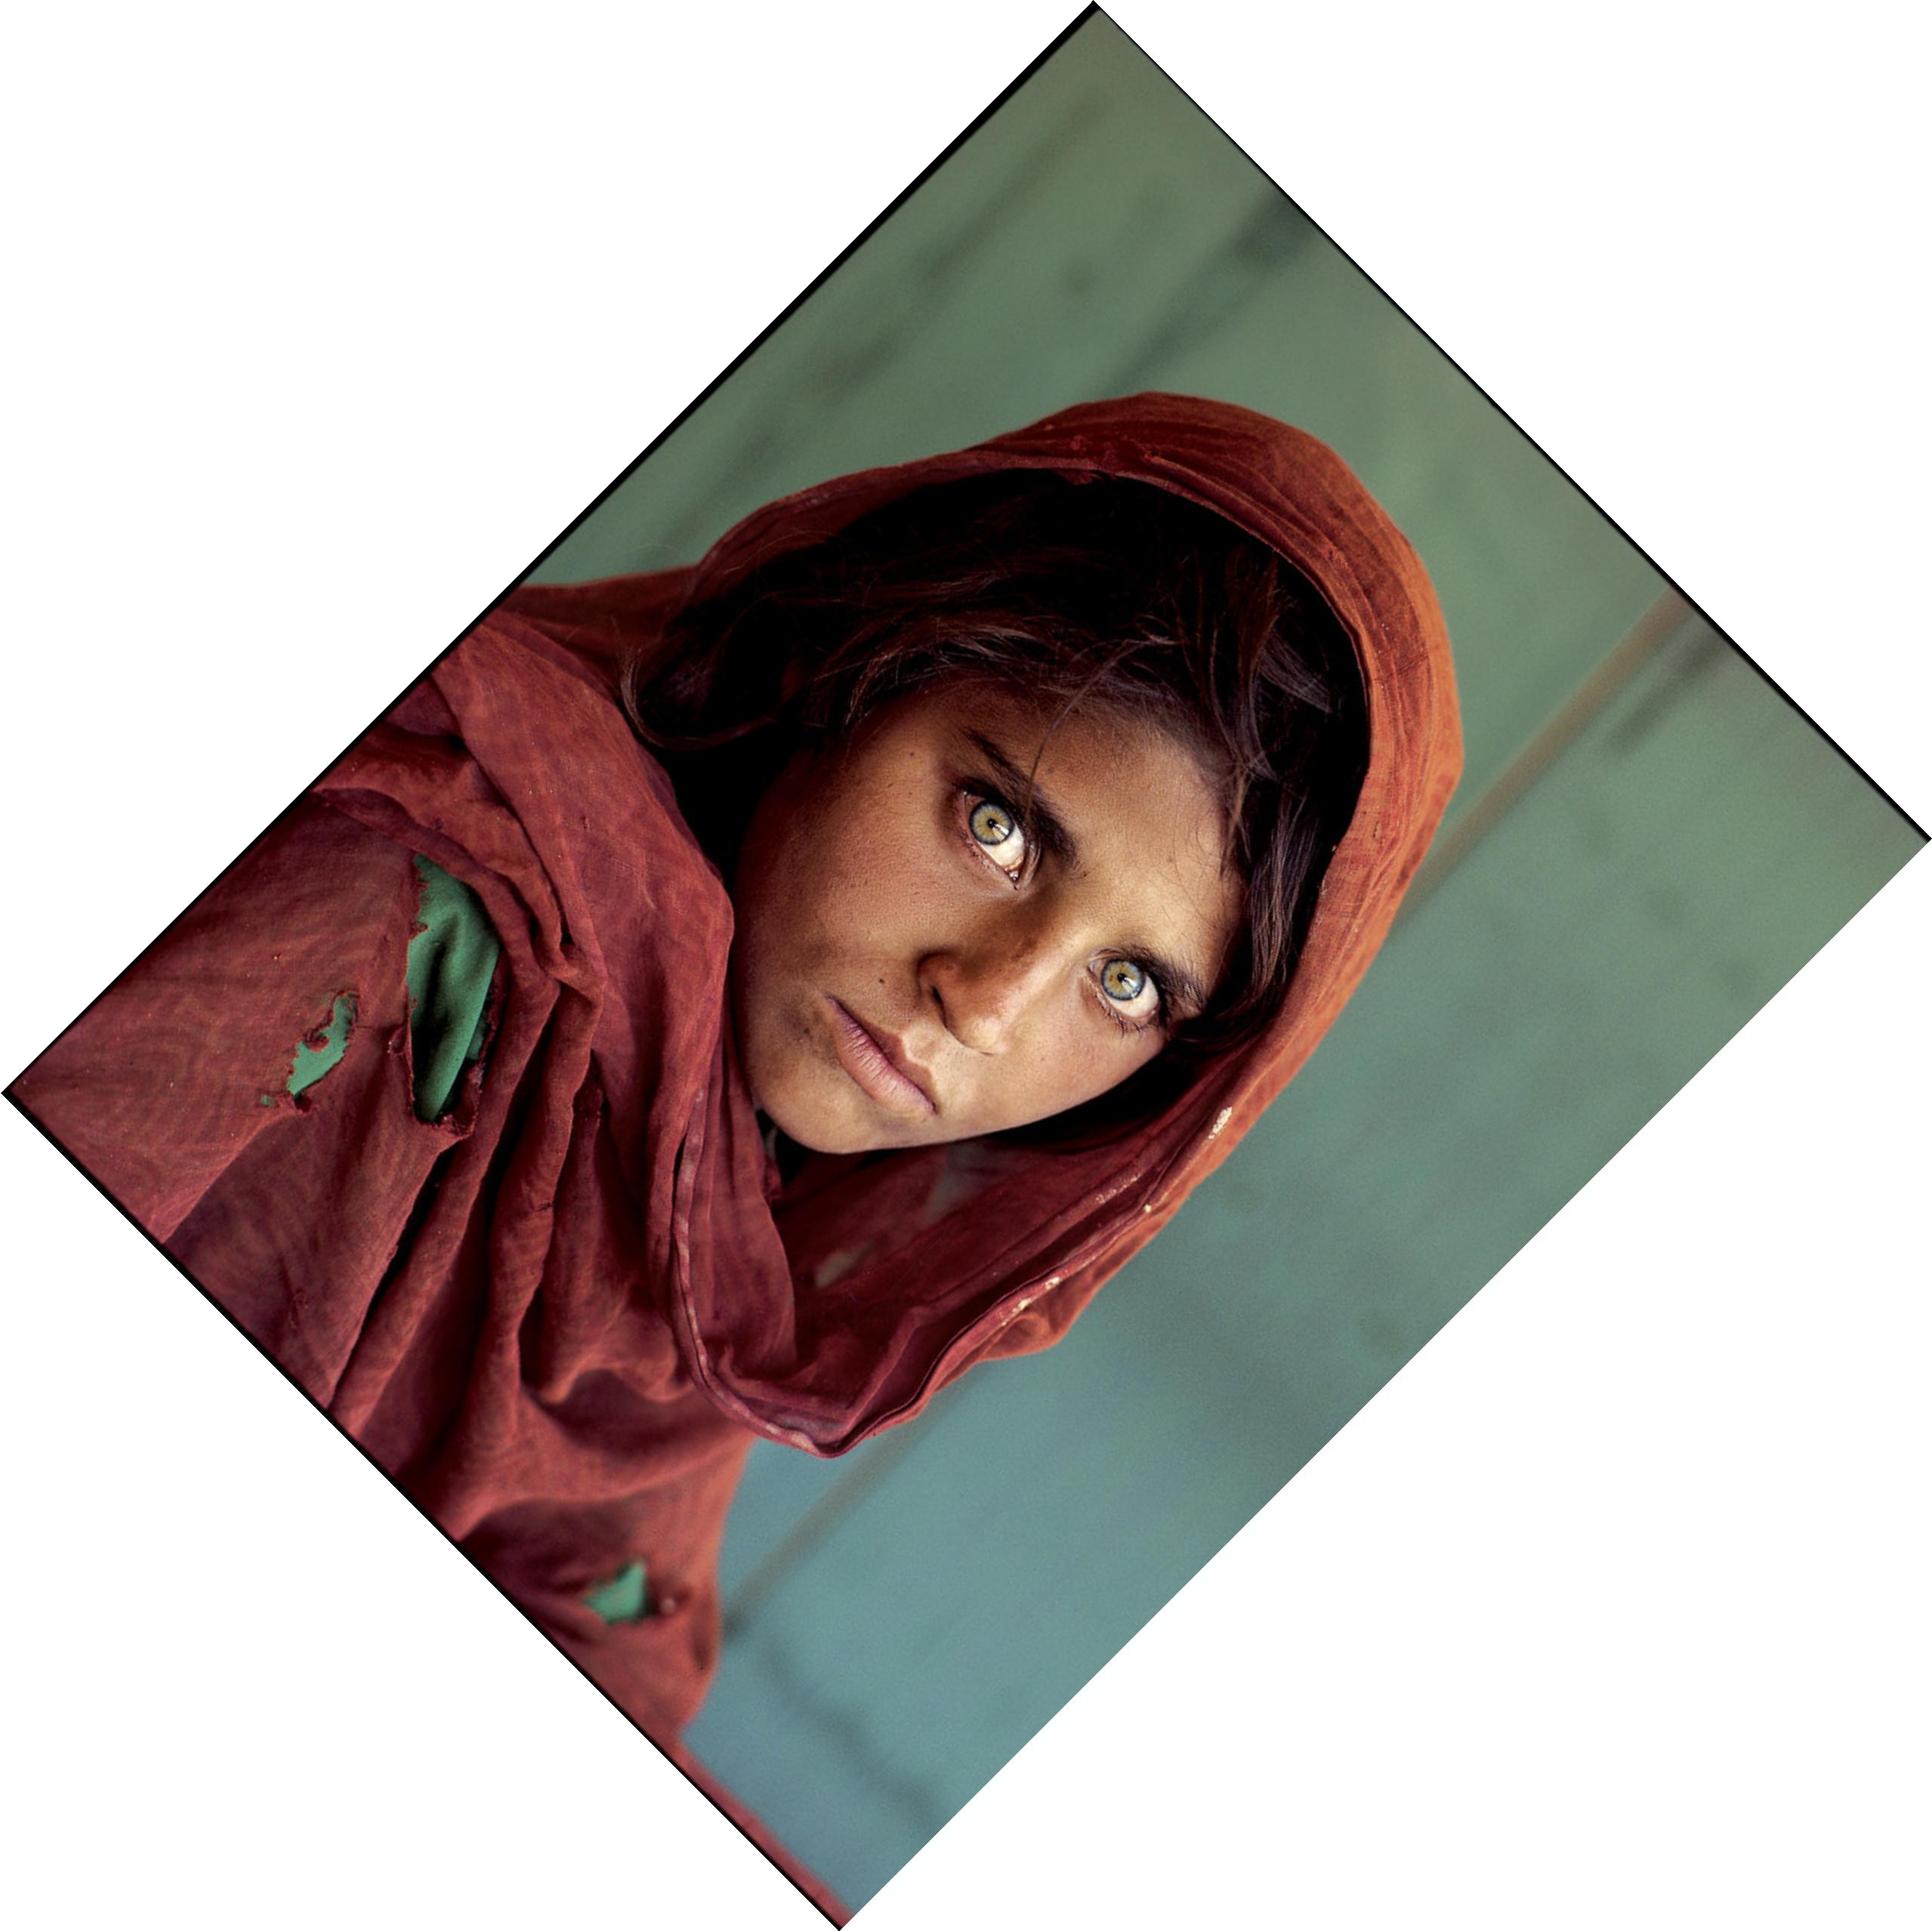
\includegraphics[scale=0.04]{q1/output/similar_2_1_2.jpg}
        \subcaption{}
    \end{subfigure}
    \begin{subfigure}{.3\textwidth}
        \centering
        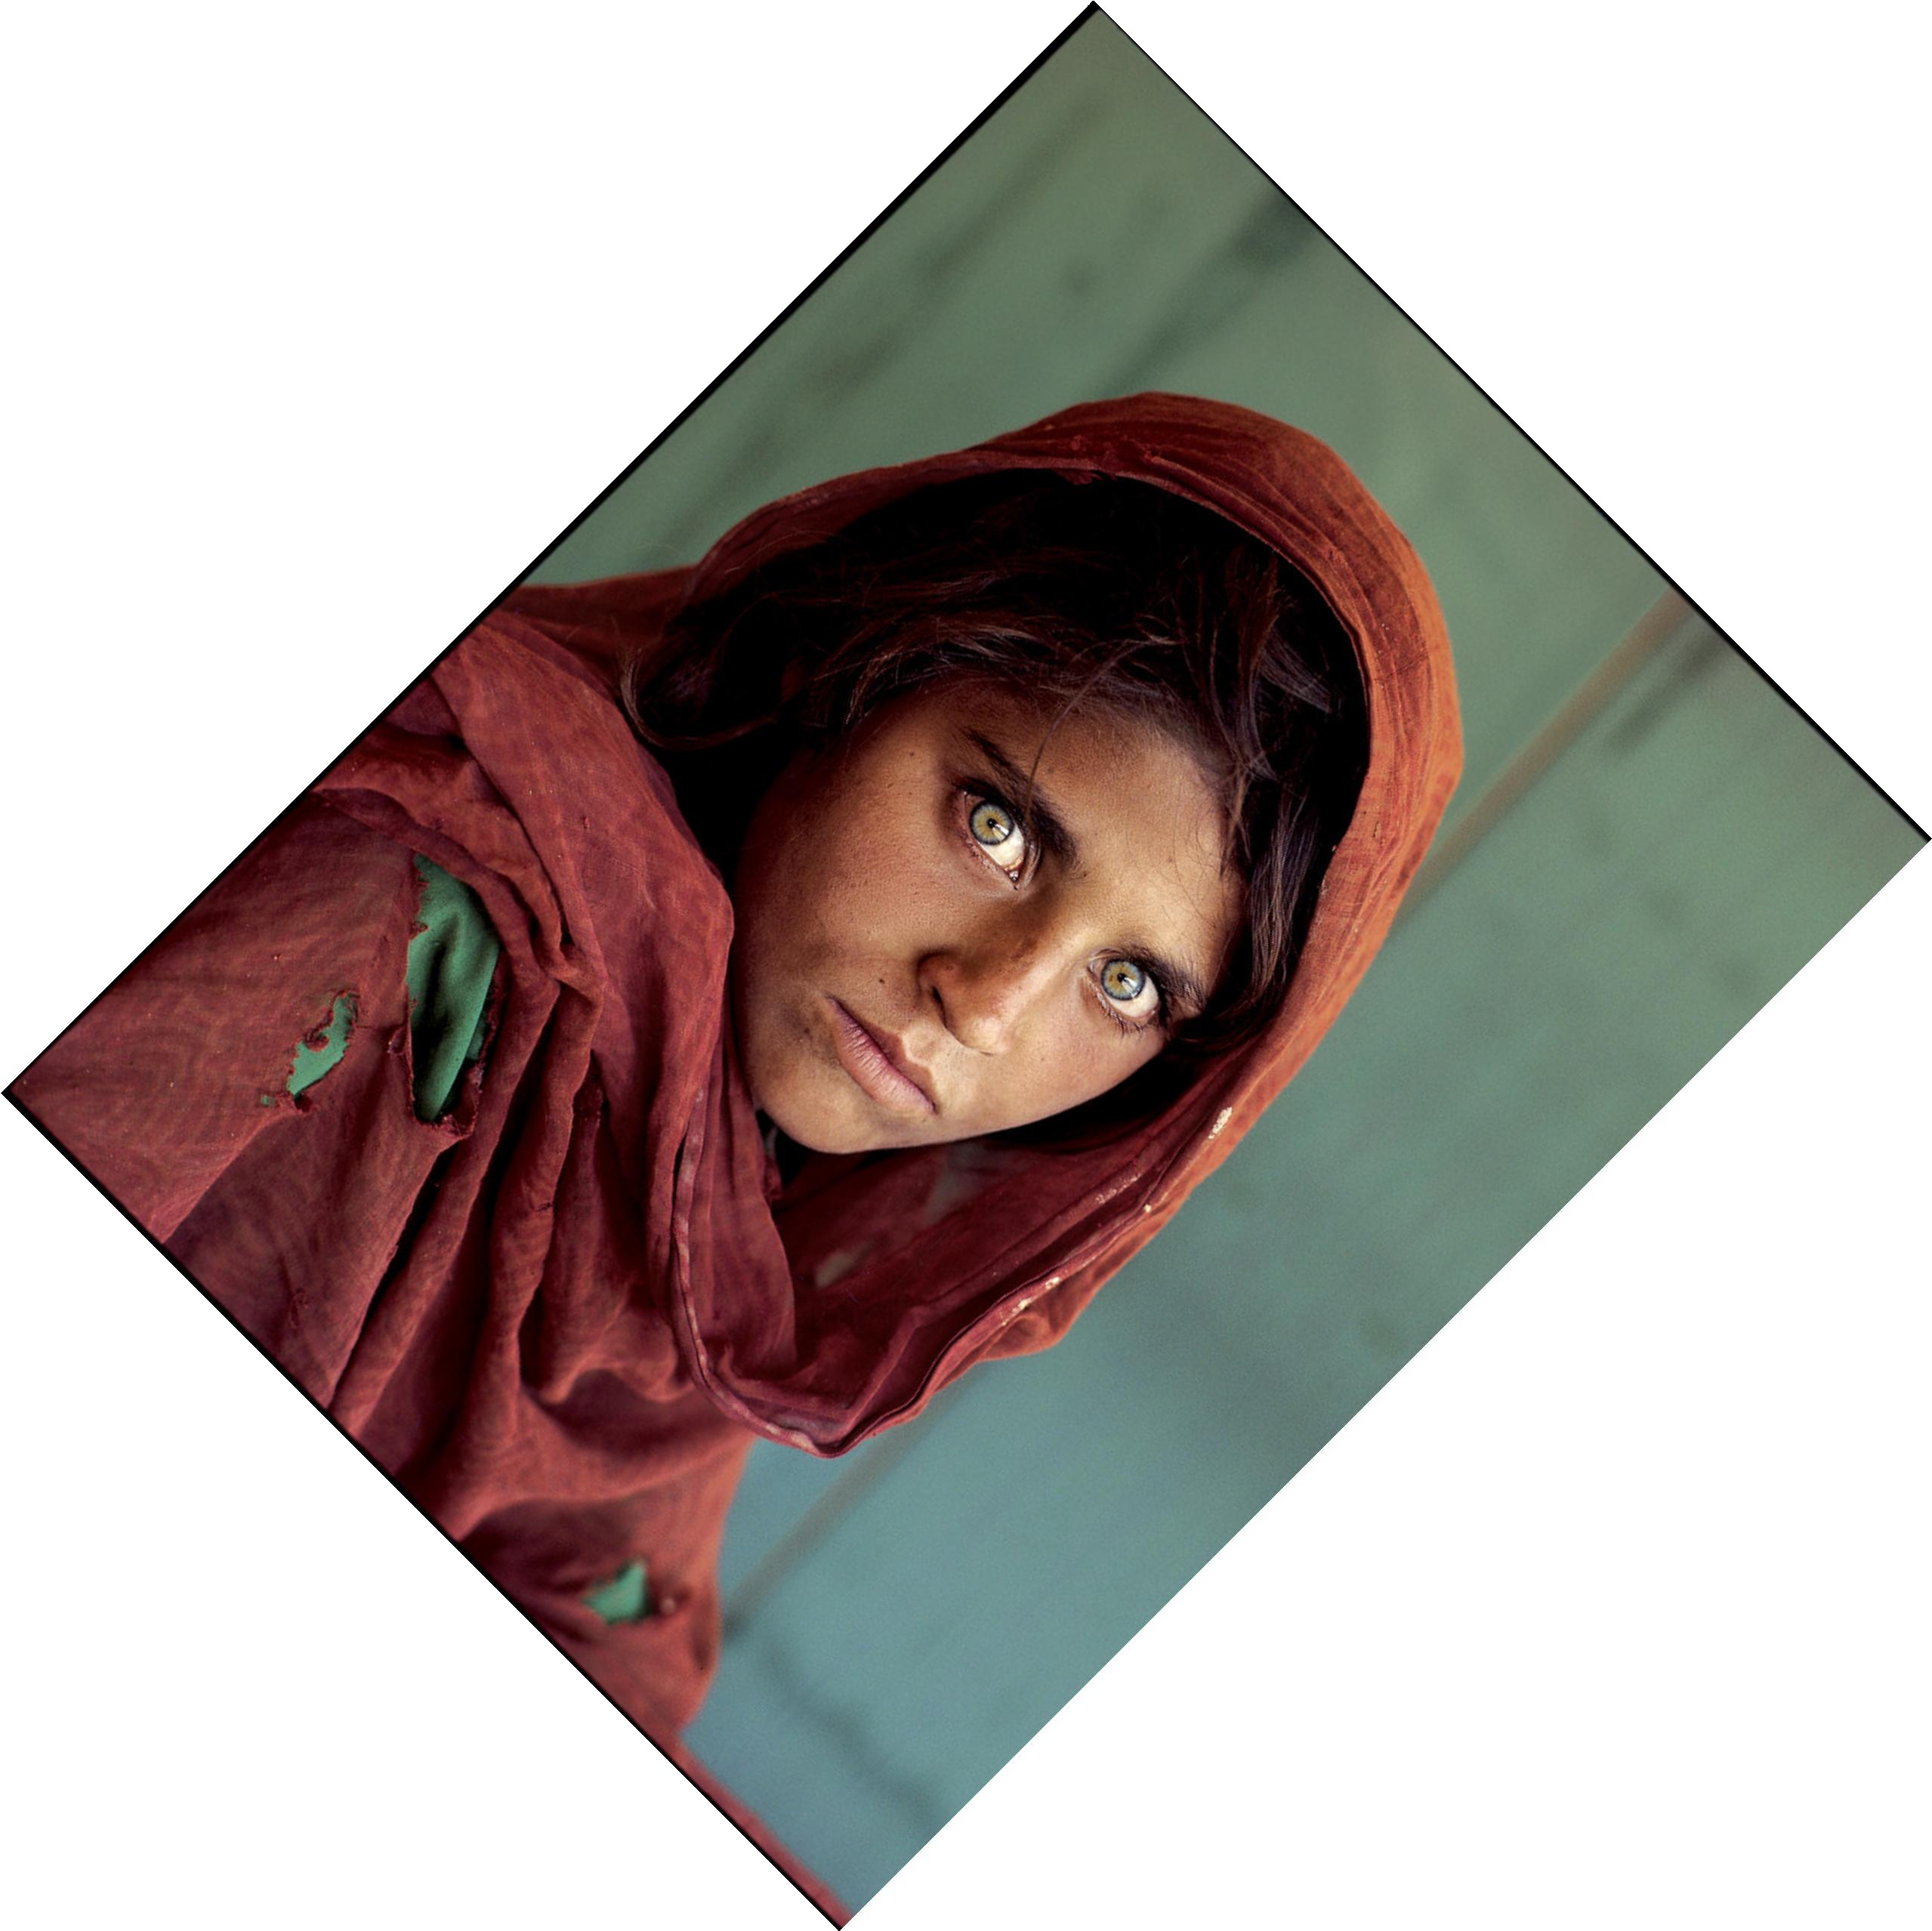
\includegraphics[scale=0.04]{q1/output/similar_2_2_2.jpg}
        \subcaption{}
    \end{subfigure}
    \caption{(a) blah (b) blah (c) blah}
\end{figure}

\subsection{Interpretation}
The \texttt{applyhomography.py} function is designed to compensate for the shift in the output image's origin. The code transforms the four corners of the input image using the homography matrix H. 
It then finds the minimum and maximum x and y coordinates. The size of the output image is then set to encompass all these points. 

\end{document}

